\chapter{Contraction Hierarchies, Hierarchical Hub Labelings}\label{chapter:ch}

\todo{Anfang der 2000x Google Maps, etc}

\section{Contraction Hierarchies}
Eine Methode um in Graphen sehr schnell kürzeste Pfade zu berechnen, sind Contraction Hierachies.
Die von \cite{geisberger2008contraction} vorgestellte Methode nutzt ein ähnliches Konzept zu der in \autoref{graphs:strassengraphen} Idee der Wichtigkeit auf und funktioniert deshalb für Straßengraphen sehr gut.
Die Grundidee der Suche eines kürzesten Pfades ist ein Bidirektionale Suche, welche jeweils relativ zum Start- und Zielknoten nur wichtigere Knoten besucht.
Durch diese Einschränkung des Suchraums kann, je nach Graphentyp, ein Speedup mehrerer Größenordnungen erreicht werden.

\subsection{Kontraktion}

Der Name Contraction Hierachies leitet sich aus Konzept der Knoten Kontraktion (contraction) ab.

\begin{definition}[Knoten Kontraktion]
    Sei $G = (V, E)$ ein Graph. Sei $v \in V$ der zu kontraktierende Knoten. Die Kontraktion von $v$ erfolgt durch:

    \begin{enumerate}
        \item\label{ch:contraction:when_shortcut}
        Für jeden Vorgänger $u \in V$ und jeden Nachfolger $w \in V$ von $v$ wird, wenn $v$ auf dem einzigen kürzesten Pfad zwischen $u$ und $w$ liegt, eine Abkürzungskante (Shortcut) $(u, w, w_{uw})$ zu $E$ hinzugefügt.

        \item
              Alle Kanten von und zu $v$ entfernt werden.
    \end{enumerate}
\end{definition}

Nach der Kontraktion $v$ ist also isoliert.
Um die Abkürzungen zu erzeugen, kann von jedem Vorgänger eine modifizierte Dijkstra zu allen Nachfolgern ausgeführt werden, bei der keine Kanten von und zu $v$ begangen werden.
Ist die Länge der potenziellen Abkürzung kürzer als die der in de modifizierten Dijkstra Suche gefunden Pfad, so liegt $v$ auf dem einzigen kürzesten Pfad zwischen $u$ und $w$.
Diese Kontraktion erhält für die verbleibenden Knoten die kürzesten Pfaddistanzen.

Betrachten wir dies wieder am Beispielgraph.
Sei $i$ der zu kontraktierende Knoten, die Nachbarn sind $a$, $b$, $j$ und $h$.
Die kürzesten Pfade von $\{a, b\}$, $\{b, j\}$, $\{h, j\}$ und $\{a, h\}$ führend nicht durch $i$.
Der kürzeste Pfad zwischen $\{a, j\}$ führt jedoch über $i$.
Daher wird eine Kante zwischen $a$ und $j$ eingefügt.
\autoref{graphs:fig:example_contraction} zeigt den Graphen nach der Kontraktion.

\begin{figure}[ht]
    \centering
    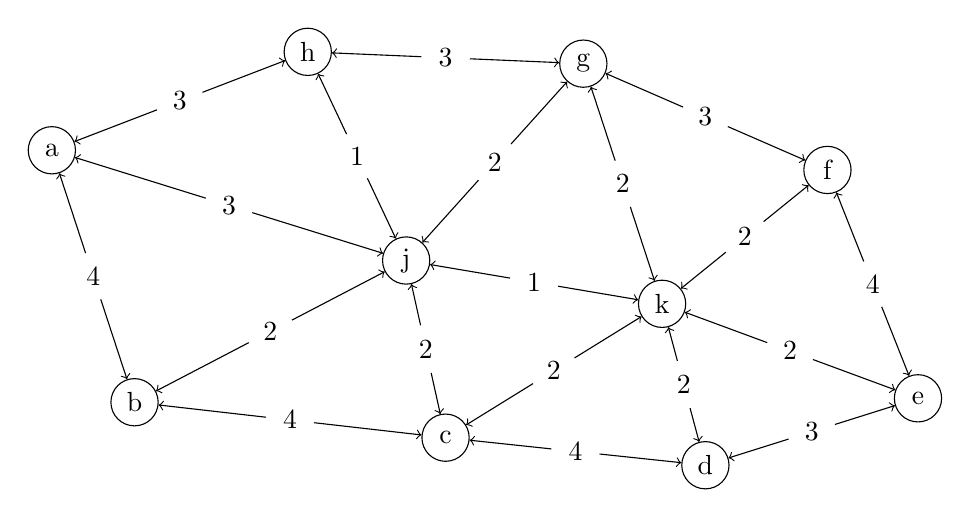
\begin{tikzpicture}
        % Nodes
        \node[circle, draw, minimum size=0.6cm, inner sep=0pt] at (0.5* 0.0, 0.5* 8.5)  (a)    {a};
        \node[circle, draw, minimum size=0.6cm, inner sep=0pt] at (0.5* 2.1, 0.5* 2.1)  (b)    {b};
        \node[circle, draw, minimum size=0.6cm, inner sep=0pt] at (0.5* 10.0, 0.5* 1.2)  (c)    {c};
        \node[circle, draw, minimum size=0.6cm, inner sep=0pt] at (0.5* 16.6, 0.5* 0.5)  (d)    {d};
        \node[circle, draw, minimum size=0.6cm, inner sep=0pt] at (0.5* 22.0, 0.5* 2.2)  (e)    {e};
        \node[circle, draw, minimum size=0.6cm, inner sep=0pt] at (0.5* 19.7, 0.5* 8.0)  (f)    {f};
        \node[circle, draw, minimum size=0.6cm, inner sep=0pt] at (0.5* 13.5, 0.5* 10.7)  (g)    {g};
        \node[circle, draw, minimum size=0.6cm, inner sep=0pt] at (0.5* 6.5, 0.5* 11.0)  (h)    {h};
        % \node[circle, draw, minimum size=0.6cm, inner sep=0pt] at (0.5* 4.0, 0.5* 6.0)  (i)    {i};
        \node[circle, draw, minimum size=0.6cm, inner sep=0pt] at (0.5* 9.0, 0.5* 5.7)  (j)    {j};
        \node[circle, draw, minimum size=0.6cm, inner sep=0pt] at (0.5* 15.5, 0.5* 4.6)  (k)    {k};


        \draw[<->]  (a) edge node[circle, fill=white] {4} (b);
        \draw[<->]  (a) edge node[circle, fill=white] {3} (h);
        \draw[<->]  (a) edge node[circle, fill=white] {3} (j);

        \draw[<->]  (b) edge node[circle, fill=white] {4} (c);
        \draw[<->]  (b) edge node[circle, fill=white] {2} (j);

        \draw[<->]  (c) edge node[circle, fill=white] {4} (d);
        \draw[<->]  (c) edge node[circle, fill=white] {2} (j);
        \draw[<->]  (c) edge node[circle, fill=white] {2} (k);

        \draw[<->]  (d) edge node[circle, fill=white] {3} (e);
        \draw[<->]  (d) edge node[circle, fill=white] {2} (k);

        \draw[<->]  (e) edge node[circle, fill=white] {4} (f);
        \draw[<->]  (e) edge node[circle, fill=white] {2} (k);

        \draw[<->]  (f) edge node[circle, fill=white] {3} (g);
        \draw[<->]  (f) edge node[circle, fill=white] {2} (k);

        \draw[<->]  (g) edge node[circle, fill=white] {3} (h);
        \draw[<->]  (g) edge node[circle, fill=white] {2} (j);
        \draw[<->]  (g) edge node[circle, fill=white] {2} (k);

        \draw[<->]  (h) edge node[circle, fill=white] {1} (j);

        \draw[<->]  (j) edge node[circle, fill=white] {1} (k);
    \end{tikzpicture}
    \caption{Beispielgraph}
    \label{graphs:fig:example_contraction}
\end{figure}

Häufig wird Kontraktionsbedingung abgeschwächt, es wird eine Kante eingefügt, wenn es \emph{wahrscheinlich} ist, dass auf dem einzig kürzesten Weg liegt.
Dazu kann eine normale Dijkstra Suche verwendet werden, es wird dann nur noch geprüft, ob der Knoten auf \emph{einem} kürzesten Pfad liegt.
Weiter kann die Anzahl der Hops der Suche begrenzt werden.

\subsection{Kontraktion}

Um die für die Beantwortung von Queries benötigte Datenstruktur, den \emph{Contracted Graph}, zu erstellen, müssen alle Knoten eines Graphens kontraktiert werden, wobei die Kanten, die in jedem Schritt entfernt werden, gesammelt werden.
Hierbei hat die Reihenfolge, in der dies geschieht einen großen Einfluss auf Perfomanz der nachfolgenden Kontraktionen und dem mit der Methode erzielte Speedup.
Die Reihenfolge der Kontraktion wird hierbei \emph{level-to-vertex} Funktion genannt, ist bijektiv und definiert als ${vtl} \colon V \to L$ mit $L \subset \mathbb{N}$, $\abs{L} = \abs{V}$ und $\max{L} = \abs{V}$.
Der Knoten mit dem niedrigsten Level wurde dabei zuerst kontrakiert.
Ihre Umkehrfunktion wird \emph{vertex-to-level} genannt.

\begin{definition}[Contrated Graph]
    Sei $G = (V, E)$ und $E'$ die durch die vollständige Kontraktion von $G$ erhalten Kanten mit der dazugehörigen vertex-to-level Funktion ${vtl}$.

    Ein Contracted Graph ist dann ein Tupel $C = (G_u, G_d)$. Der \emph{Upward Graph} $G_d$ ist dabei $G_u = (V, E_u)$ mit $E_u = \{ (t, h) \mid (t, h) \in E' \colon  {vtl}(h) > {vtl}(t) \}$, der \emph{Downward Graph} $G_d = (V, E_d)$ mit $E_d = \{ (h, t) \mid (t, h) \in E' \colon  {vtl}(h) < {vtl}(t) \}$
\end{definition}


Der Name des Upward Graphen ergibt sich daher, dass die Suche in einem Upward Graph auf das Level bezogen nur \emph{aufwärts} geht.
In \cite{geisberger2008contraction} transponieren die Autoren die Kanten des Downard Graphens nicht, daher besucht ihre Suche \emph{abwärts}.
Die Transpotion der Kanten ist hierbei nur ein Trick, damit leichter argumentiert werden kann.

\todo{Beispiel}

\subsection{Query}

Die Suche eines kürzesten Pfades von $a$ nach $e$ auf dem Beispielgraph gestaltet sich nun wie folgt:
Auf $G_u$ wird eine Dijkstra Suche von $a$ und auf $G_d$ eine Dijkstra Suche von $e$ durchgeführt.
Aus den von beiden besuchten Knoten wird derjenige ausgewählt, der die niedrigste Summe beider Distanzen hat.
\autoref{fig:ch:beispiel_suche} zeigt einen auf diese Weise gefunden Pfad auf dem Beispielgraph von $a$ nach $e$.
Es ist ersichtlich, dass die Level der Knoten auf dem Pfad zum Treffpunkt-Knoten $j$ ansteigen, bis schließlich der Knoten auf dem Pfad mit dem höchstem Level gefunden wird.
Die Kante $(a, j)$ ist hierbei ein Abkürzung, sie kürzt $i$ ab, was durch die gestrichelten Pfeile angedeuted wird.

\begin{figure}[ht]
    \centering
    \begin{tikzpicture}
        \node[circle, draw] at (0 * 1.5, -2 * 0.75)  (a)    {a};
        \node[circle, draw] at (1 * 1.5, -4 * 0.75)  (i)    {i};
        \node[circle, draw] at (2 * 1.5, -0 * 0.75)  (j)    {j};
        \node[circle, draw] at (3 * 1.5, -1 * 0.75)  (k)    {k};
        \node[circle, draw] at (4 * 1.5, -3 * 0.75)  (e)    {e};

        % draw axis
        \draw[->] (-1, -4 * 0.75) -- (-1, 0) node[above] {Level};

        \draw[->]  (a) -- (j);
        \draw[->]  (e) -- (k);
        \draw[->]  (k) -- (j);

        \draw[->, dotted]  (a) -- (i);
        \draw[->, dotted]  (i) -- (j);

    \end{tikzpicture}
    \caption{Beispiel einer Suche im Contrated Graph}
    \label{fig:ch:beispiel_suche}
\end{figure}

Algorithmus \ref{ch:query_simple} definiert dies formal.
Wie bei einer Bidirectionalen Dijkstra Suche wird der Pfad, sofern dieser existiert, aus den Teilpgaden beider Suchen erstellt.
Diese haben die Form $(u, \dotsc, t)$ bzw. $(v, \dotsc, t)$.
Um einen gültigen Pfad zu erstellen, muss $t$ aus einem dieser Teilpfade entfernt werden und der Pfad des Downward Graphens umkegehrt werden.
Anschließend können beide Pfade verkettet werden und es ensteht ein Pfad auf $C$ der Form $(u, \dotsc, t, \dotsc, v)$.
Dieser Pfad muss aber kein Pfad auf $G$ sein, da er noch Abkürzungen enthalten kann.
In \autoref{ch:subsection:pfad_gewinnung} wird darauf eingegangen, wie diese entfernt werden können.

\begin{algorithm}[ht]
    \caption{Construction Hierachies Query}
    \begin{algorithmic}[1]
        \Require Upward-Graph $G_u = (V, E_u)$, Downward-Graph $G_d = (V, E_d)$, Startknoten $s \in V$, Zielknoten $t \in V$
        \Ensure Treffknoten $m \in V \cup \{ {none} \}$, ${dist}_u$, ${pre}_u$, ${dist}_d$, ${pre}_d$
        \State ${dist}_u$, ${pre}_u$ $\leftarrow$ Dijkstra$(G_u, s)$
        \State ${dist}_d$, ${pre}_d$ $\leftarrow$ Dijkstra$(G_d, t)$

        \State
        \State $m \leftarrow {none}$
        \State $d \leftarrow \infty$
        \State

        \ForAll {$v \in V$}
        \If {${dist}_u(v) + {dist}_d(v) < d$}
        \State $m \leftarrow v$
        \State $d \leftarrow {dist}_u(v) + {dist}_d(v)$
        \EndIf
        \EndFor

        \State
        \State \Return $m$, ${dist}_u$, ${pre}_u$, ${dist}_d$, ${pre}_d$
    \end{algorithmic}
    \label{ch:query_simple}
\end{algorithm}

Die Korrektheit des Algorithmus ist nicht sofort ersichtlich, da nicht alle Kanten optimal sind und nur ein Teil aller Knoten besucht wird.
Der Beweis hierfür betrachten hierbei betrachtet einen kürzesten Pfad auf $G$ und argumentiert, warum dieser gefunden wird:

\begin{beweis}\label{ch:proof:correct}
    Der Beweis der Korrektheit folgt in zwei Schritten.

    \begin{enumerate}
        \item
              ${spd}_G ((u, v)) = d$ mit $d \neq \infty$ $\Rightarrow$ ${spd}_C((u, v)) = d$.

              Sei ${sp}((u, v))$ der kürzeste Pfad auf $G$ der unter allen kürzesten Pfaden den Knoten $t$ mit dem höchstem Level enthält.
              Erstelle aus diesem Pfad $(u, \dotsc, v)$ zwei Pfade: $(u, \dotsc, t)$ und $(v, \dotsc, t)$.

              Gehe durch $(u, \dotsc, t)$ und entferne alle Knoten, die einen niedrigeren Level als ihr Voränger haben.
              Die Tupel benachbarten Knoten im neu enstanden Pfad sind nach der Definition des upward Graph Kanten von $G_u$, und zwar solche, die ein optimales Kantengewicht haben.
              Daher wird $t$ im upward Graph mit optimaler Distanz gefunden.

              Analog dazu wird im Pfad $(v, \dotsc, t)$ mit $G_d$ argumentiert.

              Da $t$ in beiden Suchen mit optimalen Gewicht gefunden wird und auf dem kürzesten Pfad liegt, ist auch die optimale Distanz des kürzesten Pfades gefunden

        \item
              ${spd}_G ((u, v)) = \infty$ $\Rightarrow$ ${spd}_C((u, v)) = \infty$.

              Angenommen, es würde ein Pfad $(u, \dotsc, v)$ in C gefunden werden.
              Sei $t$ wieder der Knoten mit den höchstem Level auf diesem Pfad.

              Erstelle aus $(u, \dotsc, v)$ zwei Pfade: $(u, \dotsc, t)$ und $(v, \dotsc, t)$.
              Die Tuple benachbarter Knoten entsprechen wieder Kanten im Upward. bzw. Downward Graph.
              \todo{Gegenbeweis sauber führen}
    \end{enumerate}

    Daher gilt, die Suche der kürzesten Pfad Distanz in $C$ ist äquivalent zu der in $G$
    \qed
\end{beweis}

\subsection{Erstellung des Pfades}\label{ch:subsection:pfad_gewinnung}
Der in $C$ gefundene Pfad kann bisher noch Abkürzungen enthalten.
Damit der Pfad auch auf $G$ gültig ist, müssen diese ersetzt werden.
Hierfür ist eine Funktion notwendig, welche diese ersetzt.

\begin{definition}[Abkürzungsfunktion]
    Sei $G = (V, E)$ ein Graph, und $C = (G_u, G_d)$ ein Contracted Graph von $G$.
    Betrachte die Abkürzungen $(u, v)$ aus $C$ als Pfade.
    $S \coloneq V \times V \to V \cup \{ {none} \}$ ist eine \emph{Abkürzungsfunktion} von $C$, wenn eine endliche, rekursive Anwenden von $S$ auf die Abkürzungen einen gültigen Pfad in $G$ erzeugt.
\end{definition}

Um diese Funktion zu erhalten, müssen die Abkürzungen, welche beim Kontraktieren des Graphens eingefügt werden, mitsamt dem übersprungenen Knoten gesammelt werden.
Das rekursive Ersetzten kann durch den Algorithmus \ref{ch:alg:shortcut_replacement} verwirklicht werden.

\begin{algorithm}[ht]
    \caption{Shortcut replacement}
    \begin{algorithmic}[1]
        \Require Pfad $p$ mit Abkürzungen, Abkürzungungsfunktion $S \colon V \times V \to V \cup \{ {none} \}$
        \Ensure Pfad $p'$ ohne Shortcuts

        \If {$\text{len}(p) == 1$}
        \State \Return $p$
        \EndIf
        \State

        \State $p' \leftarrow ()$
        \State

        \While {$\text{len}(p) >= 2$}
        \State $w \leftarrow \text{pop}(p)$
        \State $u \leftarrow \text{pop}(p)$
        \State $v \leftarrow S((u, w))$
        \State

        \If {$v \neq none$}
        \State $\text{push}(p, u)$
        \State $\text{push}(p, v)$
        \State $\text{push}(p, w)$
        \Else
        \State $\text{push}(p, u)$
        \State $\text{push}(p', w)$
        \EndIf
        \EndWhile

        \State
        \State $p' \leftarrow \text{reversed}(p')$

        \State
        \State \Return $p'$
    \end{algorithmic}
    \label{ch:alg:shortcut_replacement}
\end{algorithm}

\subsection{Early stop}

Bisher werden beiden Suchen vollständig ausgeführt.
Die Anzahl der besuchten Knoten hierbei ist zwar kleiner als im zugrundeliegenden Graphen, jedoch ist es trotzdem wünschenswert, wenn die Suche frühzeitig gestoppt werden könnte.

Bei einer bidirectionalen Dijkstra Suche reicht es aus, die Suche zu stoppen, sobald die Summer der kleinsten Abstände der Vorwärtwarteschlange größer als der kleinste gefundene Abstand ist.
Dies ist hier nicht hinreichend, das die Suche auf im Upward bzw. Downward Graph keinen \emph{Ball} in $G$ bildet.
Anders ausgedrückt, es ist nicht garantiert, dass sich die Suchen an ihrer Front treffen:
Es ist möglich, dass die Suche im upward Graphen einen Knoten trifft, welcher selbst und alle seiner Nachfolger bereits expandiert worden sind.
Daher kann die Suche erst gestoppt werden, wenn die kleinste Distanz beider Warteschlangen größer oder gleich der des bisher besten Treffpunkt-Knotens ist.

Dies stopt die Suche zwar fühzeitig, die Anzahl der expandierten Knoten, nachdem der beste Treffpunkt-Knoten gefunden wurde ist jedoch immernoch hoch.
\todo{Funke fragen: Kann man hier noch verbessern? Ich habe die Mischung CH und ALT noch nicht verstanden}.

\subsection{Stall-on-demand}

Die im upward und downard Graphen gefunden Distanzen müssen nicht optimal sein.
Für das finden einen küzesten Pfades sind jedoch nur die Knoten interesannt, deren Distanz optimal ist.
Es ist möglich den Suchraum durch \emph{stall-on-demand} zu verkleinern.
\todo{Funke nochmal die Details. Mache ich das gerade richtig?}


% https://cstheory.stackexchange.com/questions/23767/why-is-label-pruning-possible-with-hub-labeling
Aus dieser Definition folgt, dass der kürzeste Pfad zwischen zwei Knoten in $G_u$ ist also mindestens genausolang ist wie in $G$.
Der Pfad darf aber auch länger sein.

\todo{Zeiche zwei Suchbäume, jeweils in G und Gu}

Für die Suche sind aber nur Knoten interesannt, die tatsächlich kürzesten Pfad Abstand haben.

Wie kann man diese Knoten nun leicht rausfiltern?
Beim expanded eines Knoten prüft man, für die Nachbarn der Gegenrichtung:


\subsection{Erstellung}

Die Erstellung des Contrated Graphens kann auf zwei Wegen geschehen: Durch Kontraktion und Brute-Forcing.
Inwiefern letzter eine sinnvolle Option ist wird \todo{Results} zu sehen sein.

\paragraph{Top-Down}

Bei der Top-Down Kontraktion ist die level-to-vertex Funktion ${ltv}$ vorgegeben.
Die Knoten werden in Reihenfolge ihres Levels kontrakiert, wobei mit dem niedrigsten Level begonnen wird.

\subparagraph{Zufällig sortiert}
Die Knoten werden zufällig auf die Level verteilt. \todo{Funke fragen}

\subparagraph{Sortiert nach Grad}
Die Knoten werden nach ihrem Grad sortiert, wobei die kleinsten Grade zuerst kontraktiert werden.
Die überlegung dahinter ist, dass Knoten mit vielen Nachbarn auch viele neue Kanten einfügen können, was vermieden werden soll.


\paragraph{Bottom-Up}

Bei der Bottom-Up contraction wird die vertex-to-level Funktion ${vtl}$ währen der Kontraktion erstellt.
Dafür wird mit einer Heuristik der jeweils nächst \emph{unwichtigste} Knoten ausgewählt, kontraktiert und dem nächstem Level zugewiesen.
Ein unwichtiger Knoten hat hierbei einen niedrigen Heuristik-Wert.
Die in der Praxis am meist-verwendeten Heurisiken beinhalten die \emph{Kanten-Differenz}.
Sie gibt an wie sich die Anzahl der Kanten im gesammten Graph durch die Kontraktion verändert.
Sie wird durch die Anzahl der neu hinzugefügten Kanten subtrahiert durch die Anzahl der entfernten Kanten gebildet.
Die Kontraktion eines Knoten kann dabei die Heurisitk-Werte anderer Knoten verändern.
Damit jedes mal der Knoten mit der niedrigsten Heuristik ausgewählt wird, müssen nach jeder Kontraktion alle Heuristik-Werte neuberechnet werden.
Dies ist im Allgemeinen jedoch zu teuer ist, weshalb in der Praxis sich zwei Methoden als effektiv gezeigt haben:

Beim \emph{Lazy poping} besteht die Annahme, dass ein Knoten nur wichtiger werden kann.
Aus der Warteschlange wird ein Knoten entnommen und geprüft, ob sein Heuristik-Wert noch gleich ist.
Wenn er noch gleich ist, wird er kontraktiert, wenn nicht wird er zurück die Warteschlange gepusht.
Dies wird wiederholt, bis schließlich ein Knoten gefunden wird.

Beim \emph{Neighbor update} werden nach der Kontraktion eines Knoten die Heuristik Werte der Nachbarn geupdated.
Es lässt sich zeigen, dass sich die Kanten-Differenz von Nachbarn zweiter Ordnung nur in Ausnahmfällen ändert. \todo{cite}
Dies hat den Vorteil, dass dies für alle Nachbarn parallisiert passieren kann.


Um die zu einem Contracted Graph dazugehörige Shortcut-Funktion zu erhalten, muss während der Kontraktion des Graphens eine Liste der Shortcuts erstellt werden.
Wird die im vorherigen Absatz erwähnte abgeschwächte Befingung verwenden, muss darauf geachtet werden, dass sich der kürzeste Shortcut zweier Knoten während der Kontraktion des Graphens mehrmals ändern kann.
Für die Shortcut-Funktion darf nur der als letzte gesetzte, beste Shortcut verwendet werden.

\section{Hub Labels}\label{chapter:hl}

Die CH Query ohne Stopbedingung erstellt jeweils den vollen Suchbaum für den Start und Zielknoten und sucht danach den Knoten mit geringester Summe der Distanzen in beiden Bäumen.
Die Idee des Label ist es, den Suchbaum des upward bzw. downard Graphenz zu speichern.
In der in \cite{abraham2011hub} vorgestellten Terminioligy wird das Label des upward Graphen \emph{forward Label} und das des downard Graphens \emph{reverse Label} genannt.
Ein kürzester Pfad wird gefunden, in dem der Knoten mit der geringsten Summe der Distanzen des forwad und reverse Labels gefunden wird.


\subsubsection{Query}

Sei $G = (V, E)$ ein Graph und ${vtl}$ eine vertex-to-level Funktion.
Dann ist $F$ die Funktion, welche einem Knoten sein Forward Label zuweist und $R$ die Funktion, die einem Knoten sein Reverse Label zuweist.
Der \emph{Hub Graph} $H = (F, E)$ ist dann die Datenstruktur, mit der schnell kürzeste Pfade gefunden werden können.
Algorithmus \ref{hl:alg:query} zeigt wie wenig Schritte dafür notwendig sind, eine kürzeste Pfad Distanz in $H$ zu finden.

\begin{algorithm}[ht]
    \caption{Hub Label Query}
    \begin{algorithmic}[1]
        \Require Forward Labels $F$, Reverse Labels $R$, Startknoten $s \in V$, Zielknoten $t \in V$
        \Ensure Treffknoten $m \in V \cup \{ {none} \}$, ${dist}_u$
        \State $f_s \leftarrow F[s]$
        \State $r_t \leftarrow F[t]$

        \State
        \State $m \leftarrow {none}$
        \State $d \leftarrow \infty$

        \ForAll {$v \in V \colon (v, d_f) \in f_s \land (v, d_r) \in r_t$}
        \If {$d_f + d_r < d$}
        \State $d \leftarrow d_f + d_r$
        \State $m \leftarrow v$
        \EndIf
        \EndFor

        \State
        \State \Return $m$, $d$
    \end{algorithmic}
    \label{hl:alg:query}
\end{algorithm}

Der Beweis für die Korrektheut folgt dem gleichen Schema wie Beweis \ref{ch:proof:correct}.

\begin{beweis}\label{hl:proof:correct}
    Der Beweis der Korrektheit folgt in zwei Schritten.

    \begin{enumerate}
        \item
              ${spd}_G ((u, v)) = d$ mit $d \neq \infty$ $\Rightarrow$ ${spd}_H((u, v)) = d$.

              Sei ${sp}((u, v))$ der kürzeste Pfad auf $G$ der unter allen kürzesten Pfaden den Knoten $m$ mit dem höchstem Level enthält.
              Da $m$ auf dem kürzestem Pfad liegt, ist auch der Pfad $(u, \dotsc, m)$ ein kürzester Pfad.
              Da $m$ das höchste Level auf dem diesem Pfad hat, ist $(m, {spd}((u, m))) \in f_s$.

              Analog dazu ist $m$ der Knoten mit höchstem Level auf dem Pfad $(v, \dotsc, t)$ in $G^T$ und damit $(m, {spd}((m, v))) \in r_v$

              Die kürzeste Pfad Distanz kann dann durch aufsummierung von ${spd}((u, m))$ und ${spd}((m, v))$ erhalten werden.

        \item
              ${spd}_G ((u, v)) = \infty$ $\Rightarrow$ ${spd}_H((u, v)) = \infty$.

              Angenommen, es würde ein Teffpunkt-Knoten $m$ mit $(m, d_f) \in f_s$ und $(m, d_r) \in r_t$ gefunden werden.
              Nach der Definition der Labels sind $d_f, d_r \in \mathbb{R}$, also endlich.
              Da aber ${spd}_G ((u, v)) = \infty$ muss $d_f = \infty$ oder $d_r \infty$ gelten.
              Daher wäre das Forward oder Reverse Label illegal.
    \end{enumerate}

    Daher gilt, die Suche der kürzesten Pfad Distanz in $H$ ist äquivalent zu der in $G$
    \qed
\end{beweis}

Die eigentliche Suche ist dann nur noch das finden des Treffpunkt-Knotens.

\todo{Wie hängen kleinstes und optimales hitting set zusammen?}

\subsection{Pfad erstellung}

Um nachdem ein Treffpunkt-Knoten $m$ gefunden wurde einen Pfad erstellen zu können sind noch zusätzliche Information notwendig.
Wie bereits erwähnt repräsentiert ein Label einen Suchbaum.
Um den Pfad auf diesen zu erstellen, muss für jeden Knoten in dem Label sein Vorgänger, falls vorhanden, bekannt sein.
Dafür wird die Label Definition von $V \times \mathbb{R}$ erweitert auf $V \times \mathbb{R} \times V$.
Der erstellte Pfad kann dann jedoch weiterhin Abkürzungen enthalten.
Diese sind jedoch gleich Art wie die des Contracted Graph, der dort verwendete Algorithmus zur Erstellung eines gültigen Pfades kann wieder verwendet werden.


\subsection{Datenstruktur}

Die HL Query ist es dann den overlapp zweier Labels zu finden.
Damit das leicht möglich ist, werden die Einträge (Vertex, Distanz, Vorgänger Index) im Label nach Vertex sortiert gespeichert.
Die Abfrage ist dann ein merge sort likes vergleichen beider Label.

Der kürzste pfad ist dementsprechend dann der Vertex mit geringster forward = backward distanz.
Der Vorgänger ist durch den Index des Voränger indtifiziert, dass sofort an die Stelle des Voränger gesprungen werden kann und nicht erst das ganze Label durchsucht werden muss.
Der Vertex, dem das Label label gehört hat keinen Vorgänger.

\begin{table}[ht]
    \centering
    \begin{tabular}{@{}llllll@{}}
        \toprule
        Index           &  & 0 & 1 & 2 & 2 \\ \midrule
        Vertex          &  &   &   &   &   \\
        Distanz         &  &   &   &   &   \\
        Vorgänger Index &  &   &   &   &   \\ \bottomrule
    \end{tabular}
\end{table}



\subsection{Erstellung}

\subsubsection{Merging}
Gibt es bereits eine CH, dann kann diese leicht in eine HL umgewandelt werden.
Für jeden Vertex wird ein Label erstellt, dass den Vertex enthält.
Vom Vertex mit dem höchstem Level zum niedrigsten Level werden die Labels der Nachbarn gemerged, wobei für duplikate unter den Vertices die niedrigste Distanz gewähl wird.

Da CH Suchbaum nicht optimal ist, ist das Label viel größer, als es sein müsste.
Um den Speicherbedarf zu verkleinern und die Geschwindigkeit zu erhöhen, sollten diese unnötigen Einträge noch entfernt weren, dies wird \emph{pruning} genant.

Werden die Label in der Reihenfolge der Level, startend mit dem höchstem Level erstellt, so können die bereits erstellten Label benutzt werden, um diese unnötigen Einträge zu indentifizieren.
Da ein Label nur Vertices mit mindestem dem gleichem Level wie sich selbst enhält sind die für diese Vertices die Label bereits erstellt.
Um zu Püfen ob ein Eintrag $(t, d_t)$ im Forward LAbel von $s$ optimal ist, wird der minimal overlapp zwischen diesem Label und dem Reverse LAbel von $t$ berechnet.
Das nennt man Boostraping.

\subsubsection{Brute force}

Analog zum Bruteforcing der CH Kanten auch das HL LAbel bebruteforced werden.
Der bereits bekannte Algorithmus wird nur wenig verändert, nur die Abbruchbedingung wird entfernt.

\todo{Beispielgraph Suche von $d$}

Ein Shortcut ist es, wenn es zwischen diesen beiden noch Knoten gibt.
Hierfür müssen wieder rekursiv alle Abkürzungen erstellt werden.